
\documentclass[a4paper,12pt]{article}

\usepackage[T1]{fontenc}
\usepackage[utf8]{inputenc}
\usepackage[english]{babel}
\usepackage{graphicx}
\usepackage{xcolor}

\usepackage[backend=biber]{biblatex}
\addbibresource{bibliography.bib}

\renewcommand\familydefault{\sfdefault}
\usepackage{tgheros}
\usepackage{csquotes}
\usepackage[defaultmono]{droidmono}

\usepackage{amsmath,amssymb,amsthm,textcomp}
\usepackage{enumerate}
\usepackage{multicol}
\usepackage{tikz}

\usepackage{float}
\restylefloat{figure}
\restylefloat{table}

\usepackage{geometry}
\geometry{total={210mm,297mm},
left=25mm,right=25mm,%
bindingoffset=0mm, top=20mm,bottom=20mm}
\linespread{1.5}

% my own titles
\makeatletter
\renewcommand{\maketitle}{
\begin{center}
\vspace{2ex}
{\normalfont \textsc{\@title}}
\vspace{1ex}
\\
\rule{\linewidth}{0.5pt}
\\
\@author \hfill \@date
\vspace{2ex}
\end{center}
}
\makeatother
%%%

% custom footers and headers
\usepackage{fancyhdr}
\pagestyle{fancy}
\lhead{}
\chead{}
\rhead{}
\lfoot{}
\cfoot{}
\rfoot{\thepage}
\renewcommand{\headrulewidth}{0pt}
\renewcommand{\footrulewidth}{0pt}
%

%%%----------%%%----------%%%----------%%%----------%%%

\begin{document}

\title{MS715 - Production Planning and Control}

\author{Gabriel Stefanini}

\date{\today}

\maketitle

\begin{abstract}
A long line of scientific endeavour addresses problems in the manufacturing and agriculture decision-making cycles. The scope of the project comprises the role of planning and control in the context of production of a good or a set of goods. Evaluating whether a production work-flow is effective or not and looking into the future and making forecasts is a very complex task for humans beings. Operations Research techniques contribute to making setting up a production and scheduling plan a more elucidated and mathematically-reasoned decision. 
In this article, a study case involves the investigation, modeling and the implementation of a master plan for a hypothetical set of goods and parameters, such as capacities and demands. A global optimal profit of \$10084000 was obtained while respecting the premises of demand, product and inventory.

\smallskip
\noindent \textbf{Keywords.} Operations Research, Production Planning, Mixed-Integer Linear Programming

\end{abstract}

\section{Case}
Understanding that departments inside a company embody an inter-dependent structure is a key element for strategic thinking and good positioning at a market. In this hypothetical case study, the mathematical model incorporates decision cycles of production, packaging, inventory and setup penalties.
Whether manufacturing a product in advance and keeping its surplus in inventory or choosing between different packaging options make a profound impact looking at the big picture. For that reason, Operations Research techniques and master plans have gained a new status of importance among top corporate executives and analysts.

In this example, the solution proposes optimal production and inventory plans with respect to described conditions of manufacturing and packing. It also considers the physical limitations of production, such as capacities and setup penalties. 

\section{Mathematical model}

The mathematical approach to the decision-making challenge is a Mixed-Integer Linear Programming (MILP) model. In this class of optimization techniques, the objective function and all inequalities relating to some condition are linear. However, the decision variables are mixed between continuous and discrete values. It is a significantly tougher problem to solve since standard approaches, such as linear relaxation, make use of a bigger set of linear sub-problems in order to solve the original problem. Modern solvers, such as CPLEX \cite{cplex} and Gurobi \cite{gurobi}, achieve results fairly quickly.

The model is part of a hypothetical production planning process of a set of products $I = A, B, C, D$ along a horizon $T$. The mathematical linear program was constructed as follows. \\

\begin{table}[H]
\centering
\begin{tabular}{|c|c|}
\hline
\textbf{Indices} & \textbf{Definition} \\
\hline 
 $i$ & Product \\
\hline
 $t$  & Planning horizon \\
 \hline
\end{tabular}
\caption{Indices}
\label{tab:indices}
\end{table}

\begin{table}[H]
\centering
\begin{tabular}{|c|c|c|}
\hline
\textbf{Parameters} & \textbf{Unit} & \textbf{Definition} 
\\
\hline
 $D_{t, i}$   & unit & Demand of product $i$ in period $t$  
 \\
\hline
$ic^P_i$      & \$ & Inventory cost of packaged product $i$ 
\\
\hline 
$ic^U_i$      & \$ & Inventory cost of unpackaged product $i$ \\
\hline 
$sc_i$         & \$ & Setup cost of product $i$     \\
\hline 
$\gamma_t$    & unit & Packaging capacity of a given period $t$   \\
\hline
$\rho_t$      & unit & Prodution capacity of a given period $t$  \\
\hline
\end{tabular}
\caption{Parameters}
\label{tab:parameters}
\end{table}

\begin{table}[H]
\centering
\begin{tabular}{|c|c|c|}
\hline
\textbf{Decision Variables} & \textbf{Unit} & \textbf{Definition} \\
\hline 
 ${\chi ^P}_{t, i}$    & unit & Packaged product $i$ in period $t$ \\
\hline
 ${\chi ^U}_{t, i}$    & unit & Unpackaged product $i$ in period $t$ \\
 \hline
 ${\iota ^P}_{t, i}$    & unit & Inventory of packaged product $i$ at the end of period $t$ \\
\hline
 ${\iota ^U}_{t, i}$    & unit & Inventory of unpackaged product $i$ at the end of period $t$ \\
\hline
 $\Theta_{t, i}$    & binary & Packaging trigger for product $i$ in period $t$ \\
\hline
\end{tabular}
\caption{Decision variables}
\label{tab:decision_variables}
\end{table}

\begin{itemize}
    \item \textbf{Objetive Function}
        \begin{equation}
            \min z = \sum_{t \in T}\sum_{i \in I}
                P_{t, i}
            +   U_{t, i} 
            +   S_{t, i}
        \end{equation}
    
        \begin{itemize}
            \item Packaged Product Cost \\ 
                $P_{t, i} = ic^P_i \cdot {\iota ^P}_{t, i}$
            \item Unpackaged Product Cost  \\
                $U_{t, i} = ic^U_i \cdot {\iota ^U}_{t, i}$
             \item Setup Cost  \\
                $S_{t, i} = sc_i \cdot \Theta_{t, i}$    
        \end{itemize}
    \item \textbf{Constraints for demand}
        \begin{equation}
             {\chi^P}_{t, i} 
                + {\iota^U}_{t-1, i} 
                - {\iota^U}_{t, i} 
                =
                {D^P}_{t, i} \qquad \forall{t, i}
        \end{equation}      
    \item \textbf{Constraints for production}
        \begin{equation}
             {\chi^U}_{t, i} 
                + {\iota^U}_{t-1, i} 
                - {\iota^U}_{t, i} 
                =
                {\chi^P}_{t, i} \qquad \forall{t, i}
        \end{equation}    
    \item \textbf{Constraints for packaging capacity}
        \begin{equation}
             \sum_{i \in I} {\chi^P}_{t, i} \leq \gamma_t  \qquad \forall{t, i}
        \end{equation}
    \item \textbf{Constraints for production capacity}
        \begin{equation}
             {\chi^P}_{t, i} \leq \rho_t  \qquad \forall{t, i}
        \end{equation}
    \item \textbf{Constraints for setup penalty}
        \begin{equation}
             {\chi^P}_{t, i} \leq \gamma_t  \cdot \Theta_{t, i}
             \quad  \forall{t, i}
        \end{equation}    
\end{itemize}

The optimization model was implemented using AIMMS \cite{aimms}. In 1993, AIMMS was introduced as a new type of algebraic modeling language (AMP). It consists of an integrated combination of a modeling language, a graphical user interface, and numerical solvers.\\


\begin{figure}[H]
\centering
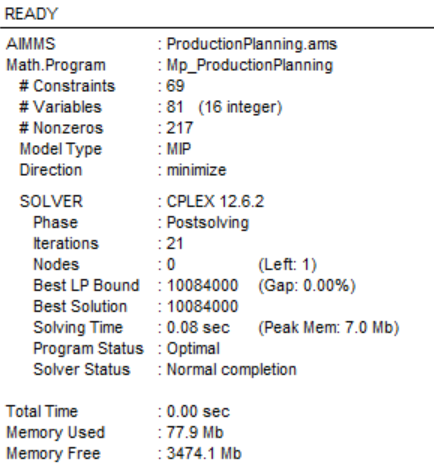
\includegraphics[scale=0.5]{1.png}
\caption{Solver on AIMMS}
\end{figure}

In light of the numerical results, which rely on a strong mathematical of and bullet-proved theory of optimality, one can argue that the best production planning to implement is already well-known. Moreover, it extends the visibility of costs and inventory capacities throughout the horizon. 

\begin{table}[H]
\centering
\begin{tabular}{|c|}
\hline
\textbf{Objective Function (\$)}  \\
\hline
10084000 \\
\hline 
\end{tabular}
\caption{Objective Function}
\end{table}

The mathematical model naturally balances out the costs while respecting the initial conditions and premises.

\begin{figure}[H]
\centering
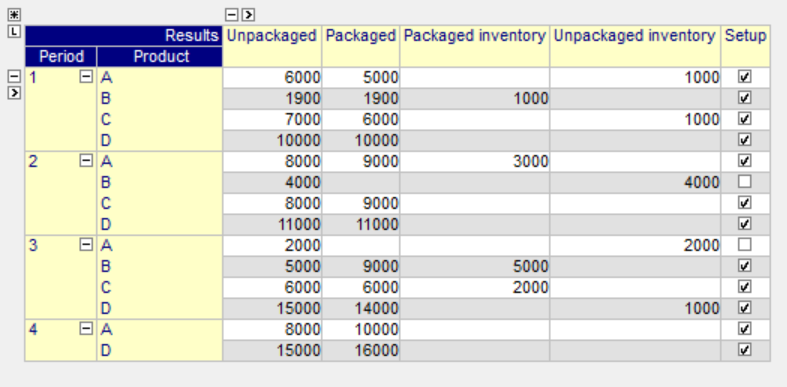
\includegraphics{2.png}
\caption{Results on AIMMS}
\end{figure}

In conclusion, the illustrated plan gives a better panorama of decision. Rather than a guess into the future, the results contribute to mathematically ensure the optimal outcome given the premises. Moreover, as computational tool, it has the capacity of parametrization and algorithmic enhancements, which implies that, in case of a turnover in the market, one will be able to predict promptly the impact and carry out asserted actions for limiting loss and identifying opportunities.

\printbibliography

\end{document}